\documentclass{article}     % Määritellään luotavan dokumentin tyyppi

\usepackage{amsmath}        % Matematiikkapaketti
\usepackage[utf8]{inputenc} % UTF-8 merkistö 
\usepackage[T1]{fontenc}    % Tuki ääkkösille
\usepackage{parskip}        % Rivinvaihto kappaleiden väliin, ei sisennystä
\usepackage{graphicx}       % Grafiikkapaketti kuvien lisäämiseen
\usepackage{epstopdf}       % Mahdollisuus lisätä *.eps tyyppisiä kuvia                          
\usepackage{textcomp}
\usepackage{ marvosym }
\usepackage[finnish]{babel}
\usepackage{listings}
\usepackage{fancyhdr}
\title{SCI-C0200 - Fysiikan ja matematiikan menetelmien studio}
\author{Hampurilaisbaarin jonon simulointi\\ \\ Osama Abuzaid 524832 \\ Joonatan Bergholm 507260}

\begin{document}                % Aloittaa dokumentin
\maketitle
\newpage

\pagestyle{fancy}
\lstset{language = Matlab}

\section*{Johdanto}

Työn tarkoituksena on selvittää Niittykummun Mc\LaTeX'in drive in -hampurilaisbaarin kassojen optimmalinen lukumäärä, kun asiakkaita mittauksen mukaan saapuu keskimäärin $\lambda = 40$ per tunti (eli $\lambda = \frac{2}{3 \mathrm{min}}$) ja yhden asiakkaan palvelimiseen menee keskimäärin 4 minuuttia. Lisäksi tiedetään, että palveluaika on eksponenttijakautunut ja että asiakkaita saapuu Poisson($\lambda$)-prosessin mukaisesti. \par
Hampurilaisbaarin, kuten minkä tahansa muunkin yrityksen omistaja, pyrkii minimoimaan kustannuksiaan heikentämättä tuotteensa tai palvelunsa tasoa, sillä silloin pystytään tekemään enemmän voittoa ja ylimääräisen kassahenkilökunnan palkkaaminen lisää kuluja, joten kassojen lukumäärä kannattaa yrittää pitää mahdollisimman pienenä. Tästä syystä ongelma on hampurilasbaarin omistajalle mielenkiintoinen. \par
Eräs tapa ratkaista tämä ongelma on Monte Carlo -simulaatio, jossa samaa satunaisuutta sisältävää simulaatiota ajetaan useita kertoja ja näiden simulaatioiden lopputuloksista kootaan lopullinen tulos. Tässä kyseissä ongelmassa voidaan ajaa samaa simulaatiota useita kertoja eri kassojen lukumäärillä ja tutkia, että kuinka monta kassaa tarvitaan, jotta jonot eivät kasva liian suuiksi.


\section*{Poisson-jakauma}

Saamme eksponentiaalisesti jakautuneen satunnaismuuttujan $t$ yhtälöstä $F(t) = R$, jossa $F$ on eksponentiaalijakauman kertymäfunktio ja $R$ on tasajakautunut satunnaismuuttuja.

\begin{align*}
F(t) =& R \\
1-e^{-\lambda t} =& R \\
-\lambda t =& \ln (1 - R) \\
t =& -\frac{1}{\lambda} \ln (1 - R)
\end{align*}

Tälloin poisson-jakauma saadaan, kun otetaan satunnaislukuja $t$ kunnes niiden summa ylittää jonkin rajan.

\section*{a}

\begin{figure}
\centering
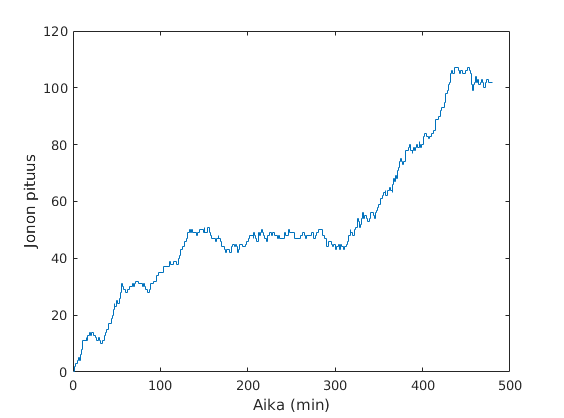
\includegraphics[width = \textwidth]{matlab/a.png}
\caption{Tilanne kun vain kaksi kassaa on käytössä.}
\label{fig:a}
\end{figure}

Kuvassa \ref{fig:a} näkyy jonon pituuden kehitys, kun vain kaksi kassaa on auki. Tämä olisi hampurilaisyrittäjän kannalta erittäin epäedullinen tilanne. Monte Carlo -simulaatiolla saadaan keskimäärin jonon pituudeksi päivän lopussa noin 83.

\section*{b}
Kassahenkilökuntaa on oltava käytettävissä vähintään sen verran, että jono ei pääse kasvamaan mielivaltaisesti. Tämä tapahtuu silloin, kun odotusarvoisesti asiakkaita tulee yhtä nopeasti sisään kuin niitä menee myös ulos. Mallin mukaan asiakkaita poistuu keskimäärin $\frac{1}{\mu_j}$ minuutissa ja autoja tulee $\lambda$ autoa aikayksikössä. Jotta jonon pitus ei pääsisi pitkällä aikavälillä kasvamaan, on oltava
\begin{align}
\max\left(\frac{1}{\mu_j}\right) &= \lambda \nonumber\\
\frac{s}{\mu} &= \lambda \nonumber\\
s &= \mu \lambda \approx 2,7.
\end{align}
Näin ollen kassahenkilökuntaa on oltava saatavilla vähintään $\lceil \mu \lambda \rceil = 3$ kappaletta, jotta jonon pituus pysyy kutakuinkin vakiona. Kuitenkin pahimpien ruuhkien varalta kannattaa olla jokunen lisäkassa käytettävissä, jotta jonojen pituudet voidaan laskea halutulle tasolle.

Kokeillaan strategiaa, jossa kassoja pidetään auki yhtä monta kuin asioivia asiakkaita on kyseisellä hetkellä, jos suinkin mahdollista. Tällöin asiakkaiden jonotusaika on triviaalisti optimaalinen. Kassojen määrää optimoidaan Monte-Carlo simulaatiolla: testataan 1000 päivän otoksella keskimääräisiä jonojen pituuksia sekä auki olevien kassojen määriä eri kassamäärillä ja valitaan näistä se, joka on kustannustehokkain ja jossa jonoja ei pääse kertymään kohtuuttoman paljon. Simulaation tulokset näkyvät kuvassa \ref{fig:montecarlo}.

\begin{figure}
\centering
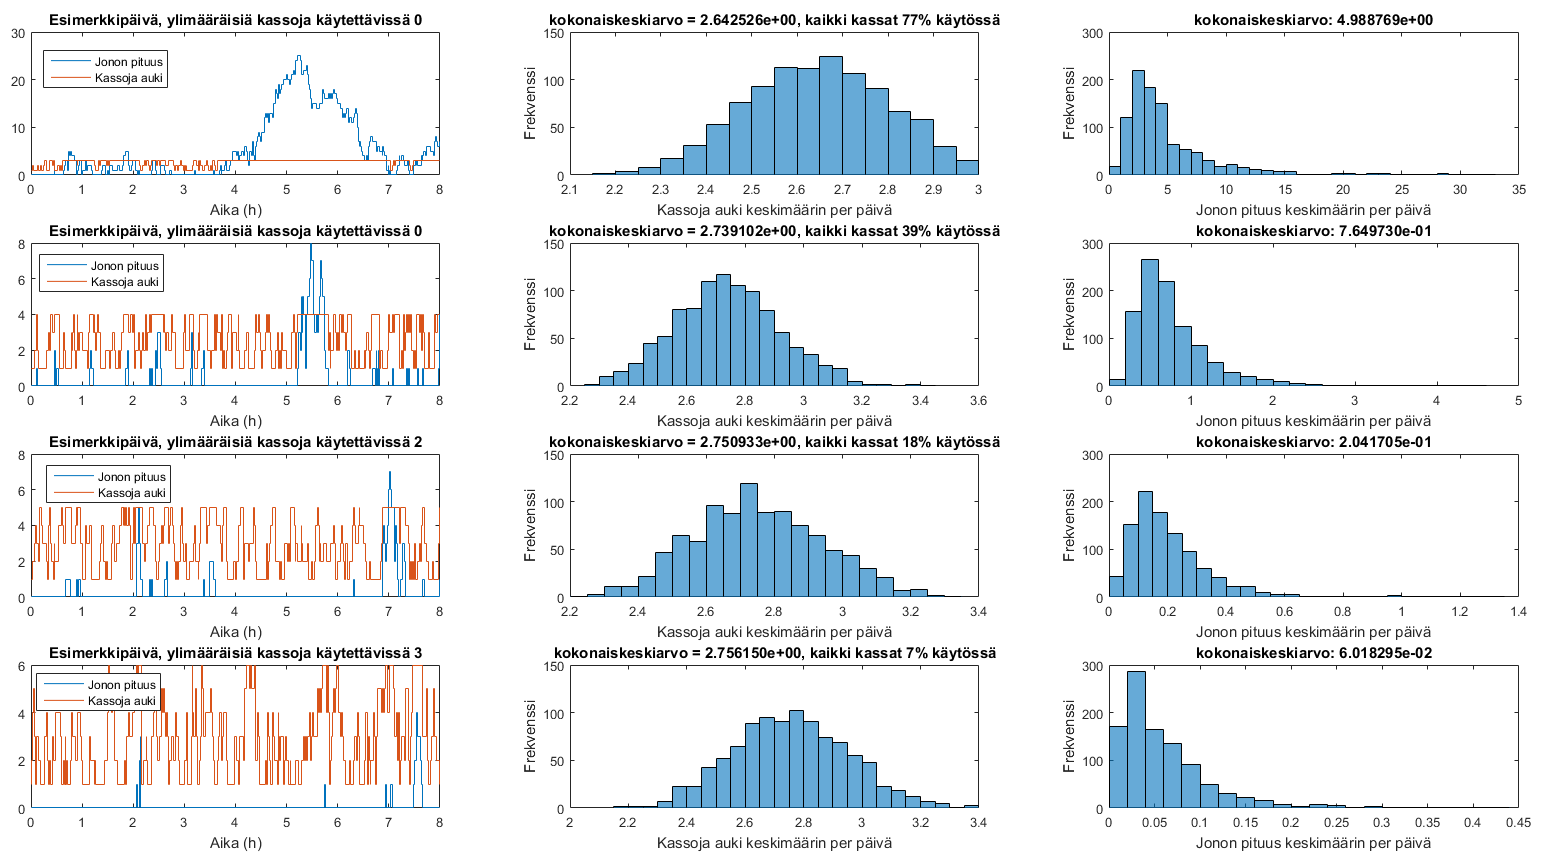
\includegraphics[width = \textwidth]{simulaatiokuvat}
\caption{Monte-Carlo simulaation tulokset. Vasemmanpuoleisimmat kuvaajat kertovat yhden päivän jononkehityksen tietyllä kassojen määrällä. Ylimääräisillä kassoilla tarkoitetaan niitä kassoja, jotka eivät ole välttämättömiä pitämään jonoa keskimäärin vakiona, ts. jos kassoja on $n$ kappaletta, on ylimääräisten kassojen lukumäärä $n - \lceil \mu\lambda \rceil$. Keskellä olevissa histogrammeissa on aukiolevien kassojen keskimääräinen määrä per päivä, otos 1000 päivää. Vastaavasti oikeanpuolimmaisssa histogrammeissa on jonon keskimääräinen pituus per päivä, otos 1000 päivää.}
\label{fig:montecarlo}
\end{figure}

Havaitaan, että ylimääräisten kassojen lisääminen ei vaikuta merkittävästi aukiolevien kassojen keskimääräiseen lukumäärään, mutta niiden vaikutus jonojen pituuteen ja erityisesti jakaumaan on merkittävä. Kun ylimääräisiä kassoje ei ole lainkaan käytettävissä, yltää jonojen keskimääräisen pituuden histogrammin häntä jopa 35 asti. Esimerkkipäivän aikaväliä 4-7h tutkailemalla nähdään hyvin miksi: jos asiakkaita tulee kerralla paljon, niin jonon pituutta ei saada lyhennettyä tehokkaasti edes täydellä kapasiteetilla, vaikkei se enää merkittävästi kasvakaan. Tämä näkyy myös siinä, että kaikki kassat on käytettävissä 77\% ajasta. Tämä oli odotettavissakin, sillä vaadittava minimikassamäärä on määritetty siten, ettei jonon pituus keskimäärin muutu miksikään.

Jonon keskimääräisen pituuden häntä lyhenee huomattavasti jo ensimmäisen ylimääräisen kassan lisäyksellä. Vaikka jonon pituus jossain vaiheessa kasvaisikin pitkäksi, niin ylimääräinen kassa pitää huolen siitä, että se myös lyhenee. Tässä skenaariossa kassoja pidetään keskimäärin auki vain n. 0,08 enemmän kuin edellisessä, mutta jonon keskimääräinen pituus lyhenee n. 85\% ja häntäkin yltää vain viiteen 35:n sijasta, joten yhden kassan lisäämisen hyöty on hyvin merkittävä tässä tilanteessa.

Kahden ylimääräisen kassan tapauksessa jonoja ei enää käytännössä ole: jonon keskimäääräisen pituuden häntä yltää vain 1,4:n asti. Kassojenkaan keskimääräinen lukumäärä ei muutu juuri miksikään edelliseen verrattuna. Kuitenkin voi kysyä, onko näin montaa kassaa järkevää ylläpitää, kun kaikki kassat ovat käytössä vain 18\% ajasta - jokainen lisäkassa nimittäin tarkoittaa lisäkustannuksia. Käytännössä siis tätä enempää kassoja ei kannata ylläpitää.

Jos itse olisin hampurilaisbaarin pitäjä, menisin yhden ylimääräisen kassan strategialla. Kassojen käyttöaste on tällöin järkevä eivätkä jonot pääse kasvamaan kohtuuttoman pitkiksi. Kassoja olisi siis tällöin 4 kappaletta.

\newpage

\appendix

\section{Yleinen lähdekoodi}

\lstinputlisting{matlab/exprand.m}
\lstinputlisting{matlab/poisson.m}
\lstinputlisting{matlab/realisation.m}

\section{Tehtävä A}

\lstinputlisting{matlab/project.m}

\section{Tehtävä B}

\end{document}              % Päättää dokumentin
